% Generated by pysimcount.pffigure -- do not edit; regenerate instead.
% figure: A-com-by-order -- Suzuki formulas of each order, r from: Commutator bound (2018)
% source: results/pf-thesis/results.json
% metric=total gatebase=cz merged
% seed=1 t=n template=simcount synth=pygridsynth
% git_commit=04cd66abb614bdc66fb48e891cef085a299e0ab1 git_dirty=False
% source_sha256=018e0b7603e6fc9f6ee358974f241415a3b93437700847b033937cc1d4250db8
% derived: A-com-by-order.tex with Lie-Trotter S1 removed by pysimcount.figdrop (Lie-Trotter S1 alone spans 45% of the original y-axis); removed legends: Lie-Trotter S1; source_sha256=66ffae439979d8fa3310b1e94cf8a5ff5a93cdf68a05c0d5b4d5f82e4692d4d2
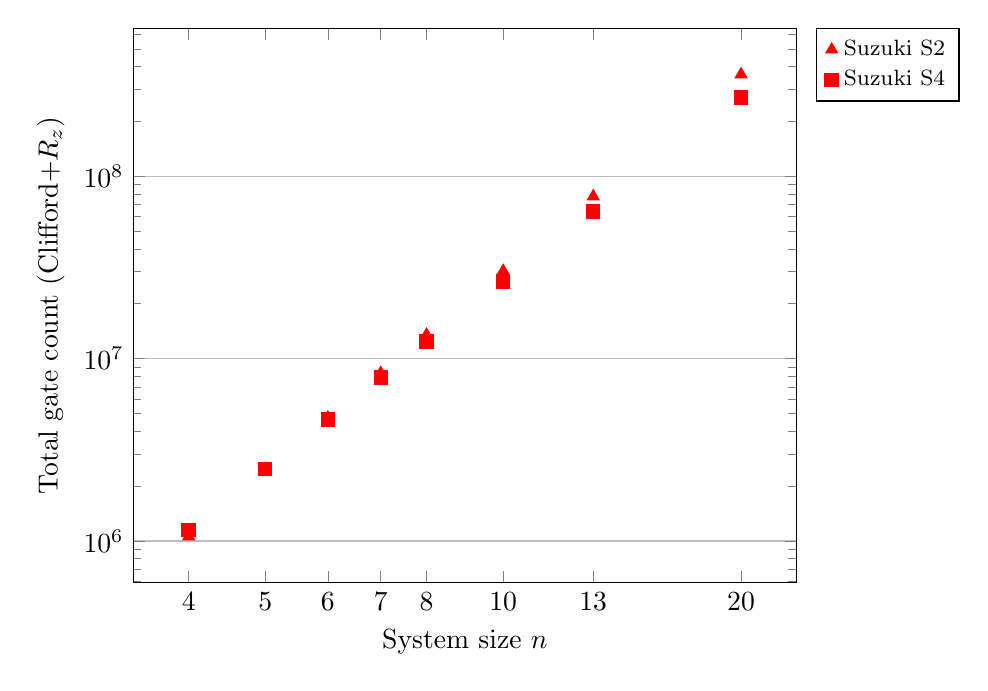
\begin{tikzpicture}
  \begin{loglogaxis}[
    width=10cm,
    xlabel={System size $n$},
    ylabel={Total gate count (Clifford+$R_z$)},
    xtick={4,5,6,7,8,10,13,20},
    xticklabels={4,5,6,7,8,10,13,20},
    ymajorgrids=true,
    legend pos=outer north east,
    legend cell align=left,
    legend style={font=\footnotesize},
  ]
    \addplot[only marks, red, mark=triangle*, mark size=2.4pt, mark options={solid, fill=red}] coordinates {
      (4,1056576)
      (5,2426400)
      (6,4743648)
      (7,8324064)
      (8,13512960)
      (10,30239040)
      (13,77585040)
      (20,361881600)
    };
    \addlegendentry{Suzuki S2}
    \addplot[only marks, red, mark=square*, mark size=2.4pt, mark options={solid, fill=red}] coordinates {
      (4,1143952)
      (5,2475100)
      (6,4635168)
      (7,7862232)
      (8,12404544)
      (10,26468200)
      (13,64126608)
      (20,270766400)
    };
    \addlegendentry{Suzuki S4}
  \end{loglogaxis}
\end{tikzpicture}
